\documentclass{officialexam} 
\usepackage{circuitikz}
\everymath{\color{blue}}
\usepackage{multirow}
\usepackage{chemfig}
\usepackage{tikz}
\usepackage{array}
\usepackage{circuitikz}
\usepackage{graphicx}
\graphicspath{ {./images/} }
\usepackage[version=4]{mhchem}
\begin{document}
	\maketitle\\
	\borderline{សំណួរ និងចម្លើយ លើមេរៀនរូបវិទ្យាទី១២}
	\begin{enumerate}[m]
		\item ចូរពោលទ្រឹស្តីសុីនេទិចនៃឧស្ម័ន?\\
		{\color{red}\sffamily ចម្លើយ}
		\begin{itemize}
			\item ម៉ូលេគុលឧស្ម័នមានចលនាឥតឈប់ឈរ និងគ្មានសណ្តាប់ធ្នាប់។
			\item ទង្គិចរវាងម៉ូលេគុល និងធុងផ្ទុកវាជាទង្គិចខ្ទាត។
			\item សន្មតនៅចន្លោះពេលទង្គិច ម៉ូលេគុលមានចលនាត្រង់ស្មើ។
			\item តម្លៃមធ្យមនៃថាមពលសុីនេទិចរបស់ម៉ូលេគុលអាស្រ័យនឹងសុីតុណ្ហភាព។
			\item គេចាត់ទុកម៉ូលេគុលឧស្ម័ននីមួយៗ ជាចំណុចរូបធាតុ។
		\end{itemize}
		\item តើច្បាប់ទី១ ទែម៉ូឌីណាមិចសិក្សាអំពីអ្វី? ចូរពោលច្បាប់នេះ។\\
		{\color{red}\sffamily ចម្លើយ}
		\begin{itemize}
			\item ច្បាប់ទីមួយទែម៉ូឌីណាមិចសិក្សាអំពីៈ បម្លែងថាមពលកម្តៅ ទៅជាកម្មន្ត ឬថាមពលបែបផ្សេងៗទៀត។
			\item ពោលច្បាប់ទី១ទែម៉ូឌីណាមិចៈ ក្នុងបម្លែងទែម៉ូឌីណាមិច កម្តៅស្រូបដោយប្រព័ន្ធ $Q$ ស្មើនឹងផលបូកកម្មន្តដែលបង្កើតដោយប្រព័ន្ធ $W$ និងបម្រែបម្រួលថាមពលក្នុងនៃប្រព័ន្ធ $\Delta U$ គេបានៈ \fbox{$Q=\Delta U+W$}។
		\end{itemize}
		\item ដូចម្តេចដែលហៅថាប្រព័ន្ធ?\\
		{\color{red}\sffamily ចម្លើយ}: ប្រព័ន្ធៈ គឺជាវត្ថុ ឬសំណុំវត្ថុដែលគេលើកមកសិក្សាធៀបទៅនឹងនឹងវត្ថុដ៏ទៃទៀត(មជ្ឈដ្ឋានក្រៅ)។
		\item ដូចម្តេចដែលហៅថាប្រព័ន្ធទែម៉ូឌីណាមិច?\\
		{\color{red}\sffamily ចម្លើយ}: ប្រព័ន្ធទែម៉ូឌីណាមិចៈ គឺជាប្រព័ន្ធដែលទទួលបម្លែងទែម៉ូឌីណាមិចអាចចេញពីភាពដើមមួយទៅភាពស្រេចមួយតាមដំណើរប្រព្រឹត្តទៅខុសៗគ្នា។
		\item ដូចម្តេចដែលហៅថាភាពនៃប្រព័ន្ធ?\\
		{\color{red}\sffamily ចម្លើយ}: ភាពនៃប្រព័ន្ធជាសំណុំលេខដែលវាសតាមទំហំរូបវិទ្យាសម្រាប់សម្គាល់លក្ខណៈរបស់ប្រព័ន្ធនៅខណៈណាមួយ។
		\item ដូចម្តេចដែលហៅថាបម្លែងទែម៉ូឌីណាមិច?\\
		{\color{red}\sffamily ចម្លើយ}: បម្លែងទែម៉ូឌីណាមិចៈ ប្រព័ន្ធមួយទទួលបម្លែងទែម៉ូឌីណាមិច កាលណាវាផ្លាស់ប្តូរភាពដោយប្តូរតែកម្មន្ត និងកម្តៅជាមួយមជ្ឈដ្ឋានក្រៅប៉ុណ្ណោះ។
		\item ដូចម្តេចដែលហៅថាបម្លែងបិទ និងបម្លែងចំហ?\\
		{\color{red}\sffamily ចម្លើយ}:
		\begin{itemize}
			\item បម្លែងបិទៈ គឺជាបម្លែងដែលប្រព័ន្ធមានភាពដើម និងភាពស្រេចដូចគ្នា។
			\item បម្លែងចំហៈ គឺជាបម្លែងដែលប្រព័ន្ធមានភាពដើម និងភាពស្រេចខុសគ្នា។
		\end{itemize}
		\item ដូចម្តេចដែលហៅថាថាមពលក្នុងនៃឧស្ម័នបរិសុទ្ធ?\\
		{\color{red}\sffamily ចម្លើយ}: ថាមពលក្នុងនៃឧស្ម័នបរិសុទ្ធៈ គឺជាថាមពលសុីនេទិចសរុបនៃម៉ូលេគុលរបស់ឧស្ម័ន។
		\item ដូចម្តេចដែលហៅថា លំនាំអុីសូករ លំនាំអុីសូបា​ និងលំនាំអុីសូទែម?\\
		{\color{red}\sffamily ចម្លើយ}:
		\begin{itemize}
			\item លំនាំអុីសូករៈ គឺជាលំនាំដែលមាឌនៃប្រព័ន្ធក្នុងពេលបម្លែងទែម៉ូឌីណាមិចមានតម្លៃថេរ។
			\item លំនាំអុីសូបាៈ គឺជាលំនាំដែលសម្ពាធនៃប្រព័ន្ធក្នុងពេលបម្លែងទែម៉ូឌីណាមិចមានតម្លៃថេរ។
			\item លំនាំអុីសូទែមៈ គឺជាលំនាំដែលមាឌនៃប្រព័ន្ធក្នុងពេលបម្លែងទែម៉ូឌីណាមិចមានតម្លៃថេរ។
		\end{itemize}
		\item ចូរពោលគោលការណ៍ភាពដើម និងភាពស្រេច។\\
		{\color{red}\sffamily ចម្លើយ}: គោលការណ៍ភាពដើម និងភាពស្រេចថាៈ កាលណាប្រព័ន្ធចេញពីភាពដើមទៅភាពស្រេច ដោយប្តរតែកម្មន្ត $\left(W\right)$ និងកម្តៅ $\left(Q\right)$ ជាមួយមជ្ឈដ្ឋានក្រៅ ផលបូកពីជគណិត $\left(Q-W\right)$ អាស្រ័យតែនឹងភាពដើម និងភាពស្រេច វាមិនអាស្រ័យនឹងរាងនៃបម្លែងទេ។
		\item ចូរពោលគោលការណ៍សមមូល។\\
		{\color{red}\sffamily ចម្លើយ}: គោលការណ៍សមមូលៈ កាលណាប្រព័ន្ធមួយទទួលបម្លែងបិទ ដោយប្តូរតែកម្មន្ត និងកម្តៅជាមួយមជ្ឈដ្ឋានក្រៅ៖ 
		\begin{itemize}
			\item បើវាធ្វើកម្មន្ត $\left(W>0\right)$ វាស្រូបកម្តៅ $\left(Q>0\right)$។
			\item បើវារងកម្មន្ត $\left(W<0\right)$ វាបញ្ចេញកម្តៅ $\left(Q<0\right)$។
		\end{itemize}
		\item ដូចម្តេចដែលហៅថាលំនាំអាដ្យាបាទិច?
		{\color{red}\sffamily ចម្លើយ}: គឺជាបម្លែងមួយដែលថាមពលកម្តៅមិនប្តូរជាមួយមជ្ឈដ្ឋានក្រៅ $\left(Q=0\right)$។
		\item ចូររៀបរាប់ដំណើរប្រព្រឹត្តទៅនៃសុិចកាកណូ។
		{\color{red}\sffamily ចម្លើយ}:
		\begin{itemize}
			\item ដំណាក់កាលទី១ៈ ឧស្ម័នស្រូបកម្តៅ $Q_{h}$ ពីធុងក្តៅ $T_{h}$ រីកមាឌតាមលំនាំអុីសូទែម។
			\item ដំណាក់កាលទី២ៈ ឧស្ម័នរីកមាឌតាមលំនាំអាដ្យាបាទិច។
			\item ដំណាក់កាលទី៣ៈ ឧស្ម័នបញ្ចេញកម្តៅ $Q_{c}$ ពីធុងត្រជាក់ $T_{c}$ រួមមាឌតាមលំនាំអុីសូទែម។
			\item ដំណាក់កាលទី៤ៈ ឧស្មនត្រូវបានបណ្ណែនតាមលំនាំអាដ្យាបាទិចរហូតដល់ស្ថានភាពដើមវិញ។
		\end{itemize}
		\item ដូចម្តេចដែលហៅថា ម៉ូទ័រចំហេះក្រៅ? ម៉ូទ័រចំហេះក្នុង?\\
		{\color{red}\sffamily ចម្លើយ}:
		\begin{itemize}
			\item ម៉ូទ័រចំហេះក្រៅៈ ប្រភេទម៉ូទ័រដែល ចំហេះកើតក្រៅកន្លែងកម្តៅធ្វើកម្មន្ត។\\
			{\color{red}\sffamily ឧទាហរណ៍}: ម៉ាសុីនដើរដោយចំហាយទឹក។
			\item ម៉ូទ័រចំហេះក្នុងៈ ប្រភេទម៉ូទ័រដែល ចំហេះកើតក្នុងកន្លែងកម្តៅធ្វើកម្មន្ត។\\
			{\color{red}\sffamily ឧទាហរណ៍}: ម៉ាសុីនបន្ទុះ ៤ វគ្គ ឬម៉ាសុីនបន្ទុះ ២ វគ្គ។
		\end{itemize}
		\item ចូរពោលទ្រឹស្តីបទកាកណូ? ដោយបញ្ជាក់រូបមន្តផង។
		{\color{red}\sffamily ចម្លើយ}: បើម៉ាសុីនមួយដំណើរការរវាងធុងពីរដែលមានសីតុណ្ហភាពថេរមានទិន្នផលអតិបរមា ដំណើរនេះមានភាព រេវែសុីប ហើយម៉ាសុីនទាំងអស់ដំណើរការនៅចន្លោះសីតុណ្ហភាពដូចគ្នាមានទិន្នផលដូចគ្នា។\\
		រូបមន្តៈ $e=1-\frac{T_{c}}{T_{h}}$។
		\item ចូររៀបរាប់វគ្គទាំងបួននៃម៉ូទ័របន្ទុះបួនវគ្គ។ {\color{red}\sffamily ចម្លើយ}:
		\begin{multicols}{4}
			\begin{itemize}
				\item វគ្គទី១ៈ វគ្គស្រូប
				\item វគ្គទី២ៈ វគ្គបណ្ណែន
				\item វគ្គទី៣ៈ វគ្គបន្ទុះ និងបន្ធូរ
				\item វគ្គទី៤ៈ វគ្គបញ្ចេញ។
			\end{itemize}
		\end{multicols}
		\item ចូររៀបរាប់វគ្គទាំងពីរនៃម៉ូទ័របន្ទុះពីរវគ្គ។ ​{\color{red}\sffamily ចម្លើយ}:
		\begin{multicols}{2}
			\begin{itemize}
				\item វគ្គទី១ៈ វគ្គបណ្ណែន និងបន្ទុះ
				\item វគ្គទី២ៈ វគ្គស្រូបបញ្ចូល និងបញ្ចេញ។
			\end{itemize}
		\end{multicols}
		\item ដូចម្តេចដែលហៅថារលក? តើរលកចែកចេញជាប៉ុន្មានប្រភេទ? ចូរឲ្យនិយមន័យនៃប្រភេទរលកនីមួយៗព្រមទាំងរកឧទាហរណ៍តាមប្រភេទនៃរកលកនីមួយៗមកបញ្ជាក់ផង។\\
		{\color{red}\sffamily ចម្លើយ}: រលកៈ គឺជាការបញ្ចូនថាមពលពីចំណុចមួយទៅចំណុចផ្សេងទៀតាមរយៈមជ្ឈដ្ឋានណាមួយ។រលកចែកចេញជាពីរគឺៈ
		\begin{itemize}
			\item រលកទទឹងៈ ជារលកដែលមានគន្លងកែងនឹងទិសដៅដំណាលនៃប្រភព។ {\color{red}\sffamily ឧទាហរណ៍}: រលកទឹក រលាស់រឺុស័រ ឬខ្សែយឺត។
			\item រលកបណ្តោយៈ ជារលកដែលមានគន្លងស្របនឹងទិសដៅដំណាលនៃប្រភព។ {\color{red}\sffamily ឧទាហរណ៍}: រលកសម្លេង ទាញរឺុស័រ ឬខ្សែយឺត។
		\end{itemize}
		\item ដូចម្តេចដែលហៅថាអំព្លីទុតនៃរលក?\\
		{\color{red}\sffamily ចម្លើយ}: អំព្លីទុតនៃរលកៈ គឺជាបម្លាស់ទីអតិបរមានៃអង្គធាតុធៀបនឹងទីតាំងលំនឹង។
		\item ដូចម្តេចដែលហៅថាផាសនៃរលក?\\
		{\color{red}\sffamily ចម្លើយ}: ផាសនៃរលកៈ គឺជាដំណើររង្វិលនៃវុិចទ័របង្កើតបានជាមុំមួយ។
		\item ដូចម្តេចដែលហៅថារលកជញ្ជ្រុំ?\\
		{\color{red}\sffamily ចម្លើយ}: រលកជញ្ជ្រុំៈ គឺជារលកសុីនុយសូអុីតពីរ ដែលមានអំព្លីទុត និងជំហានរលកដូចគ្នាផ្លាស់ទីតាមទិសដៅផ្ទុយគ្នា។
		\item ចូរពោលពីគោលការណ៍រលកតម្រួត។ សរសេរសមីការរលកតម្រួត។
		{\color{red}\sffamily ចម្លើយ}:\\ រលកតម្រួត ឬរលកលីនេអ៊ែរគឺជាផលបូកវុិចទ័រនៃបណ្តាចំណុចបម្លាស់ទីរលកពីរ ឬច្រើនពេលដាលឆ្លងកាត់មជ្ឈដ្ឋានតែមួយដូចគ្នា។\\
		សមីការរលកតម្រួតៈ $y=a\sin\left(\omega t+\phi\right)$\\
		ដែលៈ $a:$ ជាអព្លីទិតនៃរលកតម្រួត$\left(m\right)$\quad $\omega:$ ជាពុលសាស្យុងនៃរលក$\left(rad/s\right)$ និង $\phi:$ ជាមុំផាសដើមសមមូលនៃរលក$\left(rad\right)$។
		\item ដូចម្តេចដែលហៅថា រ៉េសូណង់? តើរ៉េណង់មានប៉ុន្មានប្រភេទ? ចូរឲ្យនិយមន័យនៃប្រភេទនីមួយៗ។
		{\color{red}\sffamily ចម្លើយ}: រ៉េសូណង់ៈ គឺជាលំអៀងរបស់ប្រព័ន្ធលំយោលនៅត្រង់អំព្លីទុតអតិបរមា និងប្រេកង់ដែលមានខួបតូច។
		គេចែករ៉េសូណង់ជាពីរប្រភេទគឺៈ
		\begin{itemize}
			\item រ៉េសូណង់ស្ទក់ៈ ជារ៉េសូណង់ដែលមានអំព្លីទុតមិនសូវខ្លាំង តែមានដែនរ៉េសូណង់ធំ។
			\item រ៉េសូណង់ឆ្មារៈ ជារ៉េសូណង់ដែលមានអំព្លីទុតខ្លាំង តែមានដែនរ៉េសូណង់តូច។	
		\end{itemize}
		\item តើអំព្លីទុតនៃរលកតម្រួត និងលំយោលដូចគ្នាដែរឬទេ? ចូរពន្យល់។\\
		{\color{red}\sffamily ចម្លើយ}: អំព្លីទុតនៃរលកតម្រួត និងលំយោលមិនដូចគ្នាទេព្រោះ
		\begin{itemize}
			\item អំព្លីទុតនៃរលកតម្រួតៈ គឺជាបម្លាស់ទីអតិបរមានៃអង្គធាតុធៀបនឹងទីតាំងលំនឹង។
			\item លំយោលៈ គឺជាចលនាខួបដែលអង្គធាតុធ្វើចលនាសងខាងទីតាំងលំនឹង។
		\end{itemize}
		\item ដូចម្តេចដែលហៅថាចលនាសុីនុយសូអុីត? តើអេ​ឡុង​កាស្យុងរបស់រលកពីរ មានតម្លៃដូចម្តេចកាលណាចលនាលំយោលសុីនុយសូអុីតពីរមានចលនាឈមផាស?
		{\color{red}\sffamily ចម្លើយ}:
		\begin{itemize}
			\item ចលនាសុីនុយសូអុីតៈ ជាចលនាមានដ្យាក្រាមនៃលំយោលជាអនុគមន៍សុីនុយសូអុីតនៃពេល(ចលនាខួប-រលក)។
			\item អេឡុងកាស្យុងរបស់រលកពីរ មានតម្លៃផ្ទុយគ្នា កាលណាលំយោលសុីនុយសូអុីតពីរ មានចលនាឈមផាស។
		\end{itemize}
		\item ដូចម្តេចដែលហៅថា បាតុភូតអាំងទែផេរ៉ង់? ហើយបាតុភូតនេះមានប៉ុន្មានប្រភេទ? {\color{red}\sffamily ចម្លើយ}:
		\begin{itemize}
			\item បាតុភូតអាំងទែផេរ៉ង់ៈ គឺជាបាតុភូតដែលកើតចេញពីរលកពីរដែលមាន $\left(a,T,\omega, \lambda, f\right)$ ដូចគ្នាដាលកាត់គ្នាក្នុងមជ្ឈដ្ឋានតែមួយ។ អាំងទែផេរ៉ង់មានពីរប្រភេទគឺៈ អាំងទែផេរ៉ង់សង់ និងអាំងទែផេរ៉ង់បំផ្លាញ។​
		\end{itemize}
		\item ដូចម្តេចដែលហៅថា បាតុភូតឌីប្រាក់ស្យុង?​{\color{red}\sffamily ចម្លើយ}:
		\begin{itemize}
			\item ឌីប្រាក់ស្យុងៈ ជាបាតុភូតដែលកើតមានឡើងកាលណារលកប្តូរទិសដៅដំណាលពេលឆ្លងកាត់រង្វះ។
		\end{itemize}
		\item ដូចម្តេចដែលហៅថា ប្រង់អាំងទែផេរ៉ង់?{\color{red}\sffamily ចម្លើយ}:
		\begin{itemize}
			\item ប្រង់អាំងទែផេរ៉ង់ៈ គឺជាខ្សែកោងអុីពែបូលដែលកាត់តាមចំណុចអំព្លីទុតអតិបរមា និងអំព្លីទុតអប្បបរមា។
		\end{itemize}
		\item ហេតុអ្វីបានជាគេធ្វើប្រអប់ត្រីវិស័យពីស្ពាន់ ឬជ័រផ្លាស់ស្ទិច? ហេតុអ្វីមិនធ្វើពីដែក? {\color{red}\sffamily ចម្លើយ}:
		\begin{itemize}
			\item គេធ្វើប្រអប់ត្រីវិស័យពីស្ពាន់ ឬជ័រផ្លាស់ស្ទិច ព្រោះស្ពាន់ និងជ័រផ្លាស់ស្ទិច វាគ្មានជម្រាប់ម៉ាញេទិច និងគ្មានឥទ្ធិពលលើទ្រនិចត្រីវិស័យ(ទ្រនិចត្រីវិស័យមានលក្ខណៈឆក់ទាញដែក)។
		\end{itemize}
		\item តើគេប្រើវិធានដៃស្តាំយ៉ាងដូចម្តេច ដើម្បីកំណត់ទិសដៅខ្សែដែនម៉ាញេទិច ករណីចរន្តត្រង់? ករណីចរន្តវង់?\\
		{\color{red}\sffamily ចម្លើយ}: ដើម្បីកំណត់ទិសដៅខ្សែម៉ាញេទិច គេប្រើវិធីដែស្តាំៈ
		\begin{itemize}
			\item ករណីចរន្តត្រង់ៈ កន្ធែកមេដៃតាមទិសដៅចរន្ត $\left(I\right)$ រួចក្តោបម្រាមទាំងបួនតាមទិសដៅដែនម៉ាញេទិច$\left(\overrightarrow{B}\right)$។
			\item ករណីចរន្តវង់ៈ ក្តោបម្រាមទាំងបួនតាមទិសដៅចរន្ត $\left(I\right)$ រួចកន្ធែកមេដៃតាមទិសដៅដែនម៉ាញេទិច $\left(\overrightarrow{B}\right)$។
		\end{itemize}
		\item ដូចម្តេចដែលហៅថាមេដែក? តើមេដែកចែកចេញជាប៉ុន្មានប្រភេទ? ចូរឲ្យនិយមន័យនៃប្រភេទនីមួយៗ ព្រមទាំងរកឧទាហរណ៍តាមប្រភេទនៃមេដែកនីមួយមកបញ្ជាក់ផង? ចូររៀបរាប់ពីលក្ខណៈសម្គាល់នៃមេដែក។\\
		{\color{red}\sffamily ចម្លើយ}: មេដែកៈ គឺជាអង្គធាតុដែលអាចឆក់ទាញដែក និងកម្ទេចដែកបាន។ មេដែកចែកចេញជាពីរប្រភេទគឺៈ 
		\begin{itemize}
			\item មេដែកធម្មជាតិ គឺជាមេដែកដែលមានស្រាប់ក្នុងធម្មជាតិ។ ឧទាហរណ៍ៈ ដែកអុកសុីតម៉ាញេទិច $\left(\ce{Fe3O4}\right)$។
			\item មេដែកសិប្បនិមិ្មត គឺជាមេដែកដែលបង្កើតដោយមនុស្ស។ ឧទាហរណ៍ៈ ម្ចុលមេដែក របារមេដែក និងមេដែករាងអក្សរ $U$។\\
			រៀបរាប់ពីលក្ខណៈសម្គាល់នៃមេដែកៈ
			\item មានរាងច្បាស់លាស់ ហើយរឹង។
			\item មានប៉ូលពីរ គឺ $S$(ត្បូង) និង $N$(ជើង)។
			\item ឆក់ខ្លាំងត្រង់ប៉ូលទាំងពីររបស់វា។
			\item អាចឆក់ដែក និងកម្ទេចដែកបាន។
		\end{itemize}
		\item តើអ្វីខ្លះជាប្រភពនៃដែនម៉ាញេទិច? តើអាំងឌុចស្យុងម៉ាញេទិចត្រូវបានគិតជាអ្វី?\\
		{\color{red}\sffamily ចម្លើយ}: ប្រភពនៃដែនម៉ាញេទិចមានៈ មេដែក ផែនដី និងចរន្តអគ្គិសនី។
		អាំងឌុចស្យុងម៉ាញេទិច ត្រូវបានគិតជាតេស្លា$\left(T\right)$។
		\item តើវិុចទ័រដែនម៉ាញេទិចត្រង់ផ្ចិតនៃសូលេណូអុីតមួយប្រែប្រួលយ៉ាងដូចម្តេច កាលណាអាំងតង់សុីតេចរន្តកើនឡើងពីរដង? កាលណាគេប្តូរទិសដៅចរន្ត?\\
		{\color{red}\sffamily ចម្លើយ}: វិុចទ័រដែនម៉ាញេទិចត្រង់ផ្ចិតនៃសូលេណូអុីតមួយប្រែប្រួលកាលណាៈ
		\begin{itemize}
			\item ចរន្តកើនឡើងពីរដង នោះដែនម៉ាញេទិចកើនពីរដងដែរ តាម $B=\mu_o \frac{NI}{l}$។
			\item ប្តូរទិសដៅចរន្ត នោះដែនម៉ាញេទិចប្តូរទិសដៅដែរ តាមវិធានដៃស្ដាំ។
		\end{itemize}
		\item ដូចម្តេចដែលហៅថា ដែនម៉ាញេទិច?\\
		{\color{red}\sffamily ចម្លើយ}: ដែនម៉ាញេទិចៈ ជាលំហដែលនៅព័ទ្ធជុំវិញមេដែក ហើយអាចបង្កើតនូវកម្លាំងម៉ាញេទិចបាន។
		\item ដូចម្តេចដែលហៅ ដែនម៉ាញេទិចឯកសណ្ឋាន? ហើយដែននេះកើតមាននៅត្រង់ណាខ្លះ?\\
		{\color{red}\sffamily ចម្លើយ}: ដែនម៉ាញេទិចឯកសណ្ឋាន គឺជាដែនម៉ាញេទិចដែលមានខ្សែដែនជាបន្ទាត់ស្របៗគ្នា មានទិស ទិសដៅដូចគ្នាអាំងតង់សុីតេស្មើគ្នាជានិច្ច។ ដែនម៉ាញេទិចឯកសណ្ឋានកើតមានៈ
		\begin{itemize}
			\item នៅខាងក្នុងសូណូអុីត។
			\item នៅចន្លោះប៉ូលទាំងពីរនៃមេដែករាង $U$។
			\item នៅចន្លោះបូប៊ីន ហុឺម-ហ៊ុល។
		\end{itemize}
		\item ដូចម្តេចដែលហៅថាអាំងឌុចតង់នៃសៀគ្វី? តើវាអាស្រ័យនឹងអ្វីហើយមានខ្នាតដូចម្តេច?\\
		{\color{red}\sffamily ចម្លើយ}: អាំងឌុចតង់ គឺជាមេគុណសមាមាត្ររវាងភ្លុចម៉ាញេទិច $\Phi$ និងចរន្ត $I$(ប្រែប្រួល)។ វាអាស្រ័យនឹងរាងធរណីមាត្រងាយរបស់បូប៊ីន ហើយមានខ្នាតគិតជា ហង់រី $\left(H\right)$។
		\item តើដែនម៉ាញេទិច និងភ្លុចម៉ាញេទិចខុសគ្នាយ៉ាងដូចម្តេច? មានខ្នាតគិតជាអ្វី?\\
		{\color{red}\sffamily ចម្លើយ}: ដែនម៉ាញេទិច និងភ្លុចម៉ាញេទិចខុសគ្នា
		\begin{itemize}
			\item ដែនម៉ាញេទិច គឺជាលំហដែលនៅព័ទ្ធជុំវិញមេដែក ហើយអាចបង្កើតនូវកម្លាំងម៉ាញេទិចបាន។ អាំងឌុចស្យុង $\left(B\right)$ មានខ្នាតគិតជា តេស្លា $\left(T\right)$។
			\item ភ្លុចម៉ាញេទិច គឺជាទំហំសម្រាប់សម្គាល់ចំនួនខ្សែដែនម៉ាញេទិចដែលឆ្លងកាត់ផ្ទៃមួយ។ ភ្លុចអាំងឌុចស្យុង $\left(\Phi\right)$ \\មានខ្នាតគិតជា វែប៊ែរ $\left(Wb\right)$។
		\end{itemize}
		\item ដូចម្តេចដែលហៅថាសូលេណូអុីត? ចូរឲ្យលក្ខណៈសម្គាល់នៃវុិចទ័រដែនម៉ាញេទិចក្នុងសូលេណូអុីត។\\
		{\color{red}\sffamily ចម្លើយ}: សូលេណូអុីតៈ គឺជាបូប៊ីនដែនមានប្រវែងជាងកាំ៥ដង $\left(l\geq 5R\right)$។ ដែនម៉ាញេទិចក្នុងសូលេណូអុីតជាដែនឯកសណ្ឋានដែលមានលក្ខណៈសម្គាល់ៈ
		\begin{itemize}
			\item ចំណុចចាប់ៈ  ត្រង់ផ្ចិតនៃសូលេណូអុីត។
			\item ទិសៈ ស្របនឹងអ័ក្សសូលេណូអុីត។
			\item ទិសដៅៈ កំណត់តាមវិធានដៃស្ដាំ។
			\item ម៉ូឌុលៈ $B=\mu_0 nI=\mu_{0}\frac{N}{l}I$។
		\end{itemize}
		\item ចលនាផង់ផ្ទុកបន្ទុកអគ្គិសនីផ្លាស់ទីក្នុងដែនម៉ាញេទិចឯកសណ្ឋាន $\overrightarrow{B}$ តើពេលណាវាមានៈ ចលនាត្រង់ ចលនាវង់ \\និងចលនាលើគន្លងស្ពៀរ៉ាល់?
		{\color{red}\sffamily ចម្លើយ}:
		\begin{itemize}
			\item ចលនាត្រង់ៈ កាលណា​ $\left(\overrightarrow{v}_{0}\uparrow\uparrow\overrightarrow{B}\right)$ ឬ $\left(\overrightarrow{v}_{0}\uparrow\downarrow\overrightarrow{B}\right)$
			\item ចលនាវង់ៈ កាលណា $\left(\overrightarrow{v}_{0}\bot\overrightarrow{B}\right)$
			\item ចលនាលើគន្លងស្ពៀរ៉ាល់ៈ កាលណា $\alpha=\left(\overrightarrow{v}_{0},\overrightarrow{B}\right)$
		\end{itemize}
		\item ដូចម្តេចដែលហៅថាស្បុិចក្រាប?\\
		{\color{red}\sffamily ចម្លើយ}: ស្បុិចក្រាប: គឺជាឧបករណ៍សម្រាប់ញែកអុីសូតូបនៃធាតុគីមី កំណត់ភាគរយនៃអុីសូតូប វាស់ម៉ាសនៃអុីសូតូបវិភាគល្បាយឧស្ម័ន ឬអង្គធាតុរឹង និងកំណត់រូបមន្តលាតនៃអង្គធាតុសមាសសីរា​ង្គ​។
		\item ដូចម្តេចដែលហៅថាបាតុភូតអាំងឌុចស្យុងអេឡិចត្រូម៉ាញេទិច?
		{\color{red}\sffamily ចម្លើយ}: ជាបាតុភូតដែលកើតមានឡើងនៅពេលដែលមានបម្រែបម្រួលដែនម៉ាញេទិច ឬបម្រែបម្រួលភ្លុចម៉ាញេទិចកើតមានក្នុងបូប៊ីន។
		\item ដូចម្តេចដែលហៅថាភ្លុចម៉ាញេទិច?\\
		{\color{red}\sffamily ចម្លើយ}: ភ្លុចម៉ាញេទិច ឬភ្លុចអាំងឌុចស្យុងៈ គឺជាទំហំសម្រាប់សម្គាល់ចំនួនខ្សែដែនម៉ាញេទិចដែលឆ្លងកាត់ផ្ទៃមួយ។
		\item ដូចម្តេចដែលហៅថាចរន្តអាំងឌ្វី?\\
		{\color{red}\sffamily ចម្លើយ}: ចរន្តអាំងឌ្វីៈ គឺជាចរន្តដែលកើតមានឡើងនៅពេលមានបម្រែបម្រួលដែនម៉ាញេទិចឆ្លងកាត់សៀគ្វី។
		\item ចូរពោលច្បាប់ឡិនដើម្បីកំណត់ទិសដៅចរន្តអាំងឌ្វី។ {\color{red}\sffamily ចម្លើយ}:
		\begin{itemize}
			\item ច្បាប់ឡិនទី១ៈ ចរន្តអាំងឌ្វីមានទិសដៅយ៉ាងណាឲ្យផលរបស់វាប្រឆាំងនឹងបុព្វហេតុអ្នកឲ្យកំណើតវា។
			\item ច្បាប់ឡិនទី២ៈ ចរន្តអាំងឌ្វីបង្កើតដែនម៉ាញេទិចថ្មីមួយដើម្បីប្រឆាំងនឹងបម្រែបម្រួលភ្លុចម៉ាញេទិចដែលឆ្លងកាត់វា។
		\end{itemize}
		\item ដូចម្តេចដែលហៅថាចរន្តភូកូល ឬចរន្តអេឌី?\\
		{\color{red}\sffamily ចម្លើយ}: ចរន្តភូកូល ឬចរន្តអេឌីៈ គឺជាចរន្តដែលកើតឡើងកាលណាភ្លុចម៉ាញេទិចឆ្លងកាត់ដុំលោហៈប្រែប្រួល។
		\item ដូចម្តេចដែលហៅថាជនិតាអគ្គិសនី?\\
		{\color{red}\sffamily ចម្លើយ}: ជនិតាអគ្គិសនីៈ គឺជាឧបករណ៍មួយដែលបម្លែងថាមពលមេកានិចទៅជាថាមពលអគ្គិសនី។
		\item ដូចម្តេចដែលហៅថាម៉ូទ័រអគ្គិសនី?\\
		{\color{red}\sffamily ចម្លើយ}: ម៉ូទ័រអគ្គិសនីជាឧបករណ៍ដែលបម្លែងថាមពលអគ្គិសនីទៅថាមពលមេកានិច។
		\item បាតុភូតអូតូអាំងឌុចស្យុងកើតមាននៅពេលណា? ចូរលើឧទាហរណ៍មួយមកបង្ហាញពីបាតុភូតនេះ។\\
		{\color{red}\sffamily ចម្លើយ}: បាតុភូតអូតូអាំងឌុចស្យុងកើតមាននៅពេលបិទ ឬពេលបើកចរន្តឲ្យរត់កាត់សៀគ្វីដែលមានបូប៊ីន ក្នុងរយៈពេលខ្លី ឬនៅពេលដែលមានបម្រែបម្រួលចរន្តឆ្លងកាត់បូប៊ីន។\\
		ឧទាហរណ៍ៈ បូប៊ីនតស៊េរី និងចង្កៀងមួយ ពេលបិទកុងតាក់ $\left(K\right)$ ចង្កៀងភ្លឺបន្តិចម្តងៗ មុននឹងភ្លឺធម្មតា ឬពេលបើកកុងតាក់ $\left(K\right)$។
		\item ដូចម្តេចដែលហៅថាបាតុភូតអូតូអាំងឌុចស្យុងអេឡិចត្រូម៉ាញេទិច?\\
		{\color{red}\sffamily ចម្លើយ}: បាតុភូតអូតូអាំងឌុចស្យុងអេឡិចត្រូម៉ាញេទិចៈ គឺជាបាតុភូតកើតមានឡើងនៅពេលដែលចរន្តប្រែប្រួលឆ្លងកាត់បូប៊ីន។
		\item ដូចម្តេចដែលហៅថាអាំងឌុចតង់នៃសៀគ្វី? តើវាអាស្រ័យនឹងអ្វីហើយមានខ្នាតដូចម្តេច?\\
		{\color{red}\sffamily ចម្លើយ}: អាំងឌុចតង់នៃសៀគ្វីៈ គឺជាមេគុណសមាមាត្ររវាងភ្លុចម៉ាញេទិច $\left(\Phi\right)$ និង ចរន្ត $\left(i\right)$(ប្រែប្រួល)។ វាអាស្រ័យនឹងរាងធរណីមាត្រងាយរបស់បូប៊ីន ហើយមានខ្នាតគិតជាហង់រី$\left(H\right)$។
		\item តើលំយោលអគ្គិសនីជាអ្វី? លំយោលអគ្គិសនីមានប៉ុន្មានប្រភេទ? អ្វីខ្លះ?\\
		{\color{red}\sffamily ចម្លើយ}: លំយោលអគ្គិសនី​ គឺជាបាតុភូតដែលកើតឡើងនៅពេលមានការបន្ទេរថាមពលពីកុងដងសាទ័រ ទៅបូប៊ីន និងការបន្ទេរថាមពលពីបូប៊ីន ទៅកុងដង់សាទ័រវិញ សារចុះ សារឡើង។\\ លំយោលអគ្គិសនីចែកចេញជាពីរប្រភេទគឺៈ លំយោលអគ្គិសនីថេរ និងលំយោអគ្គិសនីថយ។
		\item ក្នុងសៀគ្វី $\left(R,L\right)$ ក្រោយរយៈពេល $t=\tau; t=2\tau; t=3\tau; t=4\tau; t=5\tau$ និង $t=\infty$។ តើអាំងតង់សុីតេចរន្តដែលឆ្លងកាត់សៀគ្វីសម្រេចបានប៉ុន្មានភាគរយនៃចរន្តក្នុងរបបអចិន្រៃ្តយ៍?\\
		{\color{red}\sffamily ចម្លើយ}: អាំងតង់សុីតេចរន្តខណៈ $i$(ពេលបិទកុងតាក់): $i=I_{P}\left(1-e^{-\frac{t}{\tau}}\right)$
		\begin{itemize}
			\item បើ $t=\tau$ គេបាន $i=0.63I_{P}$ មានន័យថាចរន្តកើនបាន $63\%$ នៃចរន្តក្នុងរបបអចិន្ត្រៃយ៍។
			\item បើ $t=2\tau$ គេបាន $i=0.86I_{P}$ មានន័យថាចរន្តកើនបាន $86\%$ នៃចរន្តក្នុងរបបអចិន្ត្រៃយ៍។
			\item បើ $t=3\tau$ គេបាន $i=0.95I_{P}$ មានន័យថាចរន្តកើនបាន $95\%$ នៃចរន្តក្នុងរបបអចិន្ត្រៃយ៍។
			\item បើ $t=4\tau$ គេបាន $i=0.98I_{P}$ មានន័យថាចរន្តកើនបាន $98\%$ នៃចរន្តក្នុងរបបអចិន្ត្រៃយ៍។
			\item បើ $t=5\tau$ គេបាន $i=0.99I_{P}$ មានន័យថាចរន្តកើនបាន $99\%$ នៃចរន្តក្នុងរបបអចិន្ត្រៃយ៍។
			\item បើ $t=\infty$ គេបាន $i=1.00I_{P}$ មានន័យថាចរន្តកើនបាន $100\%$ នៃចរន្តក្នុងរបបអចិន្ត្រៃយ៍។
		\end{itemize}
		\item តើចរន្តឆ្លាស់ដែលងាយស្រួលក្នុងការសិក្សាជាងគេជាចរន្តអ្វី? សរសេរកន្សោមអាំងតង់សុីតេចរន្តខណៈនេះ។\\
		{\color{red}\sffamily ចម្លើយ}: ចរន្តឆ្លាស់ដែលងាយស្រួលក្នុងការសិក្សាជាងគេជាចរន្តៈ គឺចរន្តឆ្លាស់សុីនុយសូអុីត។ សមីការ $i=I_{m}\sin\left(\omega t+\phi\right)$។
		\item ដូចម្តេចដែលហៅថាចរន្តឆ្លាស់? តើវាមានភាពខុសគ្នាពីចរន្តជាប់យ៉ាងដូចម្តេចខ្លះ? តើចរន្តឆ្លាស់ផ្តល់ផលអ្វីខ្លះ? ចូរបញ្ជាក់ពីផលនីមួយៗ?\\
		{\color{red}\sffamily ចម្លើយ}: ចរន្តឆ្លាស់ជាចរន្តខួប ដែលប្តូរទិសដៅពីរដងក្នុងមួយខួប។ ចរន្នឆ្លាស់ខុសពីចរន្តជាប់ត្រង់ៈ
		\begin{itemize}
			\item ចរន្តឆ្លាស់ៈ អាំងតង់សុីតេប្រែប្រួល ហើយប្តូរទៅដៅ។
			\item ចរន្តជាប់ៈ អាំងតង់សុីតេថេរ ហើយមានទិសដៅច្បាស់លាស់។\\
			ចរន្តឆ្លាស់ផ្តល់ផលបីគឺៈ
			\item ផលកម្តៅៈ ចរន្តឆ្លាស់ប្រើឲ្យឆ្លងកាត់អង្គធាតុចម្លងអូមដើម្បីភាយកម្តៅ។
			\item ផលម៉ាញេទិចៈ ចរន្តឆ្លាស់ប្រើឲ្យឆ្លងកាត់បូប៊ីនដើម្បីបង្កើតដែនម៉ាញេទិច។
			\item ផលគីមីៈ ធ្វើអគ្គិសនីវិភាគនៃសូលុយស្យុង។
		\end{itemize}
		\item ដូចម្តេចដែលហៅថាចរន្តប្រសិទ្ធនៃចរន្តឆ្លាស់? តើវាមានទំនាក់ទំនង់ដូចម្តេចជាមួយចរន្តអតិបរមា?\\
		{\color{red}\sffamily ចម្លើយ}: ចរន្តប្រសិទ្ធនៃចរន្តឆ្លាស់ៈ ជាអាំងតង់សុីតេចរន្តជាប់ដែលឆ្លងកាត់រេសុីស្តង់ដូចគ្នាហើយក្នុងរយៈពេលដូចគ្នាមានភាយបរិមាណកម្តៅស្មើគ្នា។ មានទំនាក់ទំនង់: $I_{m}=I\sqrt{2}$។
		\item ដូចម្តេចដែលហៅថាតង់ស្យុងប្រសិទ្ធនៃចរន្តឆ្លាស់? តើវាមានទំនាក់ទំនង់ដូចម្តេចជាមួយតង់ស្យុងអតិបរមា?\\
		{\color{red}\sffamily ចម្លើយ}: តង់ស្យុងប្រសិទ្ធនៃចរន្តឆ្លាស់ៈ ជាតង់ស្យុងថេរមួយរវាងចុងទាំងពីរនៃរេសុីស្តង់សុទ្ធមួយក្នុងរយៈពេលដូចគ្នាញ្ញាំុងឲ្យមានបរិមាណកម្តៅស្មើគ្នា។ មានទំនាក់ទំនង់: $V_{m}=V\sqrt{2}$។
		\item ដូចម្តេចដែលហៅថារេសូណង់អគ្គិសនី?\\
		{\color{red}\sffamily ចម្លើយ}: គឺជាបាតុភូតដែលទទួលបានចរន្តធំបំផុត(អតិបរមា)ក្នុងសៀគ្វី។
		\item តើគេធ្វើសំណង់ប្រេណែលដើម្បីអ្វី?\\
		{\color{red}\sffamily ចម្លើយ}: គេធ្វើសំណង់ប្រេណែលដើម្បីគណនាអំព្លីទុត និងគម្លាតផាសនៃផលបូកអនុគមន៍សុីនុយសូអុីត។
		\item តើត្រង់ស្វូម៉ាទ័រ ប្រើសម្រាប់ធ្វើអ្វី? ចូរបញ្ជាក់ពីទម្រង់របស់វា?\\
		{\color{red}\sffamily ចម្លើយ}: ត្រង់ស្វូម៉ាទ័រគេប្រើសម្រាប់តម្លើង និងបន្ថយតង់ស្យុងអគ្គិសនីនៃចរន្តឆ្លាស់។\\
		ទម្រង់ត្រង់ស្វូៈ ជាបង្គុំបូប៊ីនស្នូលដែកពីរដាក់ទន្ទឹមគ្នា។
		\begin{center}
			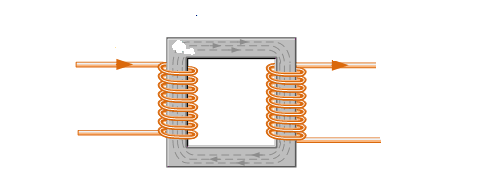
\includegraphics[scale=1.8]{image1}
		\end{center}
		\item តើក្នុងករណីណាដែលត្រង់ស្វូជាសួកវ៉ុលទ័រ និងស៊ូវ៉ុលទ័រ?
		\begin{itemize}
			\item ត្រង់ស្វួជាសួកវ៉ុលទ័រៈ  កាលណា $\frac{V_{2}}{V_{1}}=\frac{n_{2}}{n_{1}}>1$។
			\item ត្រង់ស្វួជាស៊ូវ៉ុលទ័រៈ  កាលណា $\frac{V_{2}}{V_{1}}=\frac{n_{2}}{n_{1}}<1$។
		\end{itemize}
	\end{enumerate}
\borderline{សូមឲ្យទទួលបានជោគជ័យទាំងអស់គ្នា!}\\
{\color{white}.}\dotfill
\\
{\color{white}.}\dotfill\\
{\color{white}.}\dotfill\\
{\color{white}.}\dotfill
\\
{\color{white}.}\dotfill\\
{\color{white}.}\dotfill\\
{\color{white}.}\dotfill
\\
{\color{white}.}\dotfill\\
{\color{white}.}\dotfill\\
{\color{white}.}\dotfill
\begin{center}
	\sffamily\color{blue}
	សូមសំណាងល្អ!
\end{center}\newpage
\end{document}